\documentclass[man]{apa6}
\usepackage{lmodern}
\usepackage{amssymb,amsmath}
\usepackage{ifxetex,ifluatex}
\usepackage{fixltx2e} % provides \textsubscript
\ifnum 0\ifxetex 1\fi\ifluatex 1\fi=0 % if pdftex
  \usepackage[T1]{fontenc}
  \usepackage[utf8]{inputenc}
\else % if luatex or xelatex
  \ifxetex
    \usepackage{mathspec}
  \else
    \usepackage{fontspec}
  \fi
  \defaultfontfeatures{Ligatures=TeX,Scale=MatchLowercase}
\fi
% use upquote if available, for straight quotes in verbatim environments
\IfFileExists{upquote.sty}{\usepackage{upquote}}{}
% use microtype if available
\IfFileExists{microtype.sty}{%
\usepackage{microtype}
\UseMicrotypeSet[protrusion]{basicmath} % disable protrusion for tt fonts
}{}
\usepackage{hyperref}
\hypersetup{unicode=true,
            pdftitle={Racial/Ethnic Disparities in Mental Health},
            pdfauthor={Shaina Trevino, Maria Schweer-Collins, Alejandra Garcia Isaza, \& Jonathan Pedroza},
            pdfkeywords={race, ethnicity, mental health disparities, depression, substance use},
            pdfborder={0 0 0},
            breaklinks=true}
\urlstyle{same}  % don't use monospace font for urls
\usepackage{graphicx,grffile}
\makeatletter
\def\maxwidth{\ifdim\Gin@nat@width>\linewidth\linewidth\else\Gin@nat@width\fi}
\def\maxheight{\ifdim\Gin@nat@height>\textheight\textheight\else\Gin@nat@height\fi}
\makeatother
% Scale images if necessary, so that they will not overflow the page
% margins by default, and it is still possible to overwrite the defaults
% using explicit options in \includegraphics[width, height, ...]{}
\setkeys{Gin}{width=\maxwidth,height=\maxheight,keepaspectratio}
\IfFileExists{parskip.sty}{%
\usepackage{parskip}
}{% else
\setlength{\parindent}{0pt}
\setlength{\parskip}{6pt plus 2pt minus 1pt}
}
\setlength{\emergencystretch}{3em}  % prevent overfull lines
\providecommand{\tightlist}{%
  \setlength{\itemsep}{0pt}\setlength{\parskip}{0pt}}
\setcounter{secnumdepth}{0}
% Redefines (sub)paragraphs to behave more like sections
\ifx\paragraph\undefined\else
\let\oldparagraph\paragraph
\renewcommand{\paragraph}[1]{\oldparagraph{#1}\mbox{}}
\fi
\ifx\subparagraph\undefined\else
\let\oldsubparagraph\subparagraph
\renewcommand{\subparagraph}[1]{\oldsubparagraph{#1}\mbox{}}
\fi

%%% Use protect on footnotes to avoid problems with footnotes in titles
\let\rmarkdownfootnote\footnote%
\def\footnote{\protect\rmarkdownfootnote}


  \title{Racial/Ethnic Disparities in Mental Health}
    \author{Shaina Trevino\textsuperscript{1}, Maria
Schweer-Collins\textsuperscript{1}, Alejandra Garcia
Isaza\textsuperscript{1}, \& Jonathan Pedroza\textsuperscript{1}}
    \date{}
  
\shorttitle{Racial Disparities}
\affiliation{
\vspace{0.5cm}
\textsuperscript{1} University of Oregon}
\keywords{race, ethnicity, mental health disparities, depression, substance use}
\usepackage{csquotes}
\usepackage{upgreek}
\captionsetup{font=singlespacing,justification=justified}

\usepackage{longtable}
\usepackage{lscape}
\usepackage{multirow}
\usepackage{tabularx}
\usepackage[flushleft]{threeparttable}
\usepackage{threeparttablex}

\newenvironment{lltable}{\begin{landscape}\begin{center}\begin{ThreePartTable}}{\end{ThreePartTable}\end{center}\end{landscape}}

\makeatletter
\newcommand\LastLTentrywidth{1em}
\newlength\longtablewidth
\setlength{\longtablewidth}{1in}
\newcommand{\getlongtablewidth}{\begingroup \ifcsname LT@\roman{LT@tables}\endcsname \global\longtablewidth=0pt \renewcommand{\LT@entry}[2]{\global\advance\longtablewidth by ##2\relax\gdef\LastLTentrywidth{##2}}\@nameuse{LT@\roman{LT@tables}} \fi \endgroup}


\DeclareDelayedFloatFlavor{ThreePartTable}{table}
\DeclareDelayedFloatFlavor{lltable}{table}
\DeclareDelayedFloatFlavor*{longtable}{table}
\makeatletter
\renewcommand{\efloat@iwrite}[1]{\immediate\expandafter\protected@write\csname efloat@post#1\endcsname{}}
\makeatother

\authornote{

Correspondence concerning this article should be addressed to Shaina
Trevino, 1600 Millrace Ave. Eugene, OR 97403. E-mail:
\href{mailto:strevino@uoregon.edu}{\nolinkurl{strevino@uoregon.edu}}}

\abstract{
Despite advances in access to health services, quality of care, and
overall gains in life expectancy, racial / ethnic disparities in health
in the United States persist and disproportionally affect the lives of
racial and ethnic minority groups. This project is a descriptive
approach to identifying mental health disparities for racial/ethnic
groups in the U. S. using national survey data from the Centers for
Disease Control's National Health and Nutrition Examination Survey,
2015-2016. Summary statistics and visualizations suggest the following:
(1) health disparities exist for age at onset of drug use, with those
Hispanic participants reporting the most variabilty in age of first use
of both opioids and stimulants, and (2) health disparities in depression
occurrence exist for racial/ethinic minority groups and for those
without mental healht insurance coverage. These preliminary findings
provide a rationale to prioritize funding and policy change to increase
the capacity of prevention and intervention efforts to address these
disparities.


}

\begin{document}
\maketitle

\section{Introduction}\label{introduction}

Despite advances in access to health services, quality of care, and
overall gains in life expectancy, racial/ethnic disparities in health in
the United States (U.S.) remains to disproportionally affect the lives
of racial/ethnic minority groups. D. R. Williams and Mohammed (2009)
refer to the finding of Levine et al. (2016) that approximately 100,000
African Americans who would not die if there were no racial disparities
die prematurely every year. Unfortunately, in the mental health arena,
racial/ethnic disparities are no exception.

Even though the burden and impact of physical diseases on different
racial/ethnic subgroups have been far more studied than the impact and
burden of mental health disorders, we know that globally, depression is
the leading cause of disability and loss of productivity, and that its
direst outcome, death via suicide, is on the rise (WHO, 2018). It is
well-known that mental health services are costly and thus a high
proportion of the American population cannot afford them.

Given that depression is usually screened and treated first in primary
care settings, access to medical care is the first barrier to treatment
that racial/ethnic minority groups face (D. R. Williams \& Mohammed,
2009). From there, racial/ethnic minority groups experience barriers
such as low detection rate of mental health disorders in comparison to
Whites (Borowsky et al., 2000); language barriers for non-English
speakers (Fiscella, Franks, Doescher, \& Saver, 2002); use of screening
measures not translated or validated for racial/ethnic minority groups;
issues of trust related but not limited to underrepresentation of
racial/ethnic minorities among mental health professionals, and cultural
differences in understanding and treating mental health disorders
(Miranda \& Cooper, 2004). Overall, these and other barriers affect the
access and quality of treatment racial/ethnic minority groups receive in
respect to their mental health.

Racial and ethnic minority groups in the U. S. are also
disproportionally affected by drug use disorders and carry a greater
burden of drug-overdose related deaths (Disease Control, Prevention, \&
others, 2011). Addressing these health disparities also means addressing
the social and economic conditions, which systemically reinforce these
disparities and influence individual-level drug-use behaviors. Some
evidence suggests that early-onset of drug use is predictive of poorer
drug-use outcomes in emerging and later adulthood (C.-Y. Chen, O'Brien,
\& Anthony, 2005), but few studies have examined the age of drug use
onset -- later drug use behavior relationship outside of alcohol,
tobacco and cannabis use (Anthony, Chen, \& Storr, 2005). Thus, we
choose to explore age of drug use onset for stimulants and opioids to
extend what is known about drug use health disparities.

In the present study, we aim to explore some of the health disparities
among different racial/ethnic groups using a nationally representative
sample, the National Health and Nutrition Examination Survey (NHANES)
2015 -- 2016.

\section{Methods}\label{methods}

\subsection{Participants \& Design}\label{participants-design}

The present study gathered data from the Center for Disease Control and
Prevention's (CDC) National Health and Nutrition Examination Survey
(NHANES). Using the 2015-2016 NHANES dataset, we were able to
investigate levels of depression, drug use, whether or not individuals
had insurance, if they have sought out mental health services, based on
racial/ethnic group. Data from 4,843 participants was gathered, with the
average age of participants being 32.04 (\(SD\) = 24.87) years old. The
majority of participants were women (2478), Hispanic (1573), and made
\$100,000 or more (796). Table 1 presents the breakdown of the sample
size and average age based on race/ethnicity.

\begin{table}[tbp]
\begin{center}
\begin{threeparttable}
\caption{\label{tab:apa table}Average age and sample sizes by ethnicity}
\begin{tabular}{lll}
\toprule
Ethnicity & \multicolumn{1}{c}{Age} & \multicolumn{1}{c}{N}\\
\midrule
Asian & 33.72 & 520\\
Black & 30.97 & 1012\\
Hispanic & 30.42 & 1573\\
Other/Multiracial & 22.82 & 234\\
White & 35.32 & 1504\\
\bottomrule
\end{tabular}
\end{threeparttable}
\end{center}
\end{table}

\subsection{Measures}\label{measures}

To assess depression symptoms, we used the depression module from the
full Patient Health Questionnaire (Kroenke, Spitzer, \& Williams, 2001:
PHQ). The PHQ-9 is a 9-item, self-report screening instrument.
Participants are prompted by the stem \enquote{Over the last 2 weeks,
how often have you been bothered by any of the following problems?}
Sample questions include \enquote{Feeling down, depressed, or hopeless?}
and \enquote{Thoughts that you would be better off dead or of hurting
yourself in some way}. The module uses a 4-point scale that goes from 0
(not at all) to 3 (nearly every day). \enquote{Refuse to answer} and
\enquote{Don't know} options are also included. A single score is
derived from the depression module by summing the responses for the 9
items. Scores can range from 0 to 27; higher scores reflect more severe
depressive symptoms. Insurance coverage was assessed with the item
\enquote{Are you covered by health insurance or some other kind of
health care plan?} from the NHANES Health Insurance Questionnaire.
Response choices included \enquote{Yes}. \enquote{No},
\enquote{Refused}, and \enquote{Don't know}. Usage of mental health
services was assessed with the item \enquote{During the past 12 months,
have you seen or talked to a mental health professional such as a
psychologist, psychiatrist, psychiatric nurse or clinical social worker
about your health?} from the NHANES Hospital Utilization and Access to
Care questionnaire. Response choices included \enquote{Yes}.
\enquote{No}, \enquote{Refused}, and \enquote{Don't know}. Age of first
drug use variables were assessed with single items from the NHANES Drug
Use Questionnaire (DUQ). For this study we created a composite measure
for age of first stimulant use, by averaging the items \enquote{How old
were you the first time you used cocaine, in any form?} and \enquote{How
old were you the first time you used methamphetamine?} Age of first
opioid use was assessed with the item \enquote{How old were you the
first time you used heroin?} For each of the three drug use items,
participants responded with a numerical value representing their age at
first use, ranging from 0-59 or with \enquote{I don't know.}
Participants were also permitted to refuse answering any question on the
DUQ.

\subsection{Data analysis}\label{data-analysis}

We used R (Version 3.5.1; R Core Team, 2018) and the R-packages
\emph{bindrcpp} (Version 0.2.2; Müller, 2018), \emph{dplyr} (Version
0.7.8; Wickham, François, Henry, \& Müller, 2018), \emph{forcats}
(Version 0.3.0; Wickham, 2018a), \emph{ggplot2} (Version 3.1.0; Wickham,
2016), \emph{here} (Version 0.1; Müller, 2017), \emph{kableExtra}
(Version 0.9.0; Zhu, n.d.), \emph{papaja} (Version 0.1.0.9842; Aust \&
Barth, 2018), \emph{purrr} (Version 0.2.5; Henry \& Wickham, 2018),
\emph{readr} (Version 1.2.1; Wickham, Hester, \& Francois, 2018),
\emph{rio} (Version 0.5.16; C.-h. Chan, Chan, Leeper, \& Becker, 2018),
\emph{stringr} (Version 1.3.1; Wickham, 2018b), \emph{tibble} (Version
1.4.2; Müller \& Wickham, 2018), \emph{tidyr} (Version 0.8.2; Wickham \&
Henry, 2018), and \emph{tidyverse} (Version 1.2.1; Wickham, 2017) for
all our analyses.

To explore health disparities among racial/ethnic groups, we employed a
variety of data visualizations with our variables of interest. First, we
plotted the frequency of substance use accross ethnicities according to
opioid and stimulant use. Then we plotted distributions of age of first
substance use for each ethnic group. To assess depression, we first
plotted average depression scores by ethnic group and explored the
association of age of first substance use and depression scores accross
ethnic groups by fitting a linear regression in our plot. Lastly, we
explored differences in depression scores among the racial categories
according to whether or not individuals had insurance covereage or has
reported using mental health services.

\section{Results}\label{results}

\begin{table}[tbp]
\begin{center}
\begin{threeparttable}
\caption{\label{tab:ST_table}Average depression score and age of first opioid and stimulant use by ethnicity}
\begin{tabular}{llll}
\toprule
Ethnicity & \multicolumn{1}{c}{Depression Score} & \multicolumn{1}{c}{Opioid Use} & \multicolumn{1}{c}{Stimulant Use}\\
\midrule
Asian & 3.01 & 27.86 & 21.73\\
Black & 3.16 & 22.18 & 20.30\\
Hispanic & 3.29 & 25.81 & 21.43\\
Other/Multiracial & 3.47 & 22.33 & 18.93\\
White & 3.43 & 21.60 & 20.23\\
\bottomrule
\end{tabular}
\end{threeparttable}
\end{center}
\end{table}

The average depression score and average age of first opioid and
stimulant use for each racial/ethnic group is presented in Table 2.
Briefly, White individuals had the earliest age of first use for opioids
(21.60 years). Interestingly, Asian individuals had the lowest average
depression score (3.01) and started using both opioids and stimulants
later than all other groups (mean age 27.86, 21.73 years respectively).
Individuals who reported another race or multiracial reported the
earliest age of first use for stimulants (18.93 years) and highest
reported depression score (3.47).

\subsection{Disparities in opioid and stimulant
use}\label{disparities-in-opioid-and-stimulant-use}

In our sample, 215 participants reported either opioid or stimulant use.
To explore racial/ethnic disparities in reported use, we plotted the
number of individuals who reported using opioids and/or stimulants based
on their racial category. As shown in Figure 1, more Hispanic
participants reported opioid and stimulant use, whereas Asian
participants had the lowest reported frequency of use for both
substances. To further explore disparities in substance use, we
visualized the age of first use by ethnicity (see Figure 2). This plot
shows that across both substance types Hispanic individuals have the
most variability in their age of first use. Additionally, Asian
participants have much more variability in their age of first opioid use
compared to stimulants. This observation is slightly observed among
Black and White individuals. Overall, it seems that the majority of
participants reported their age of first use to be between ages 15-25
for both substance types. However, it is more pronounced for reported
stimulant use.

\begin{figure}
\centering
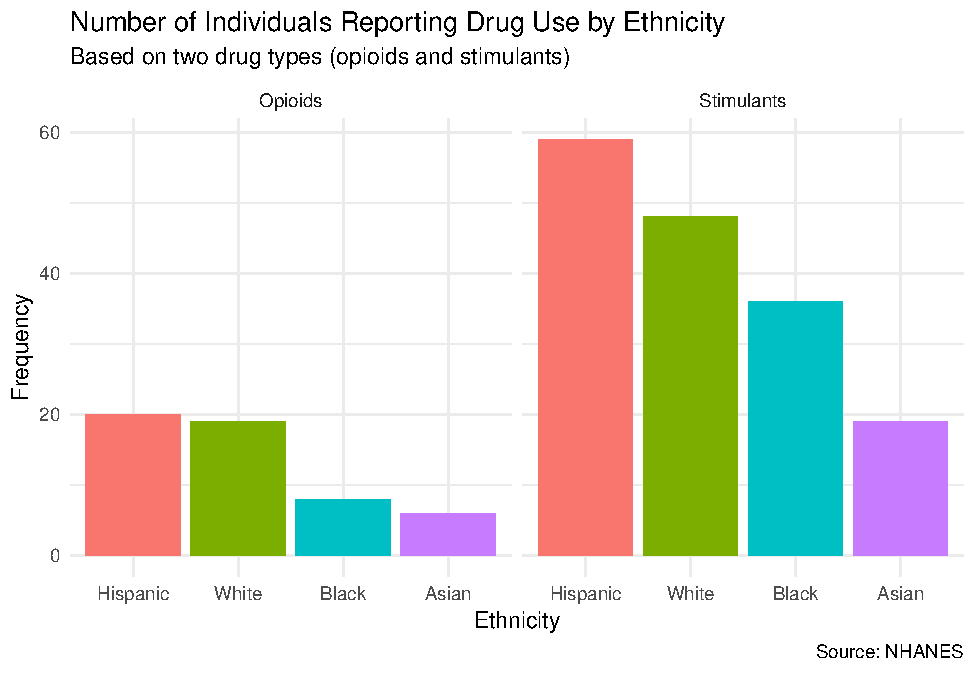
\includegraphics{Final_Paper_Group_3_files/figure-latex/ST_fig1-1.pdf}
\caption{}
\end{figure}

\begin{figure}
\centering
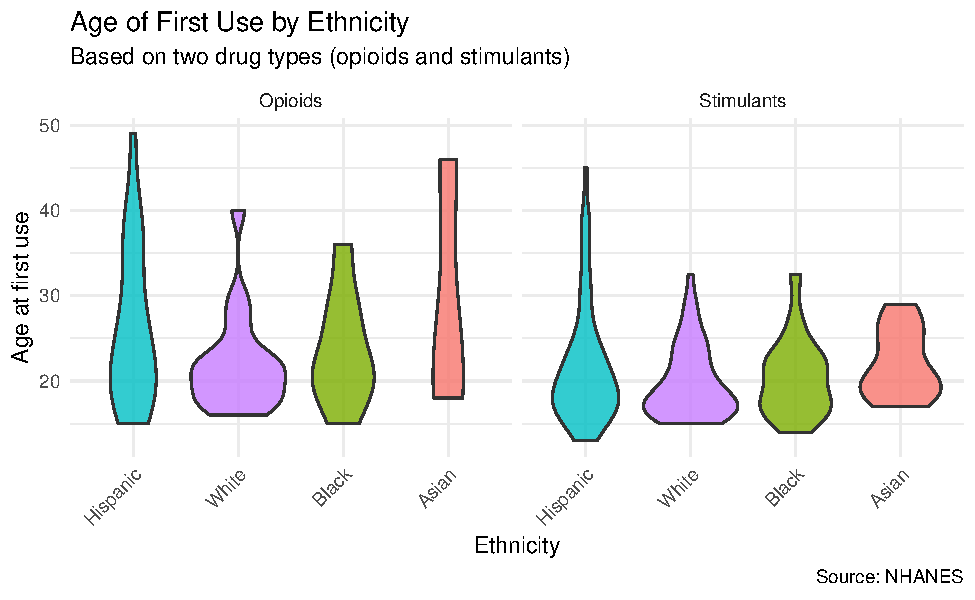
\includegraphics{Final_Paper_Group_3_files/figure-latex/ST_fig2-1.pdf}
\caption{}
\end{figure}

Since depression and substance are strongly linked in the literature, we
also produced a plot to explore racial disparities in average depression
scores by substance type. As you can see in Figure 3, Asian individuals
that reported stimulant use had the highest reported average depression
score compared to all other groups. For opioids, White participants had
the highest reported depression score. To further explore the relation
between age of first substance use and depression, we graphed age of
first use by the total depression score and faceted by substance type.
Then, we overlaid a best fit linear regression onto the graph according
to racial groups (see Figure 4). Interestingly, the plot suggests that
there is a positive association between age of first opioid use and
depression for Black individuals and a negative association for all
other racial groups. Additionally, we observed a positive relationship
between age of first stimulant use and depression for all racial groups,
however the slope of the relationship was more robust for Asian
individuals.

\begin{figure}
\centering
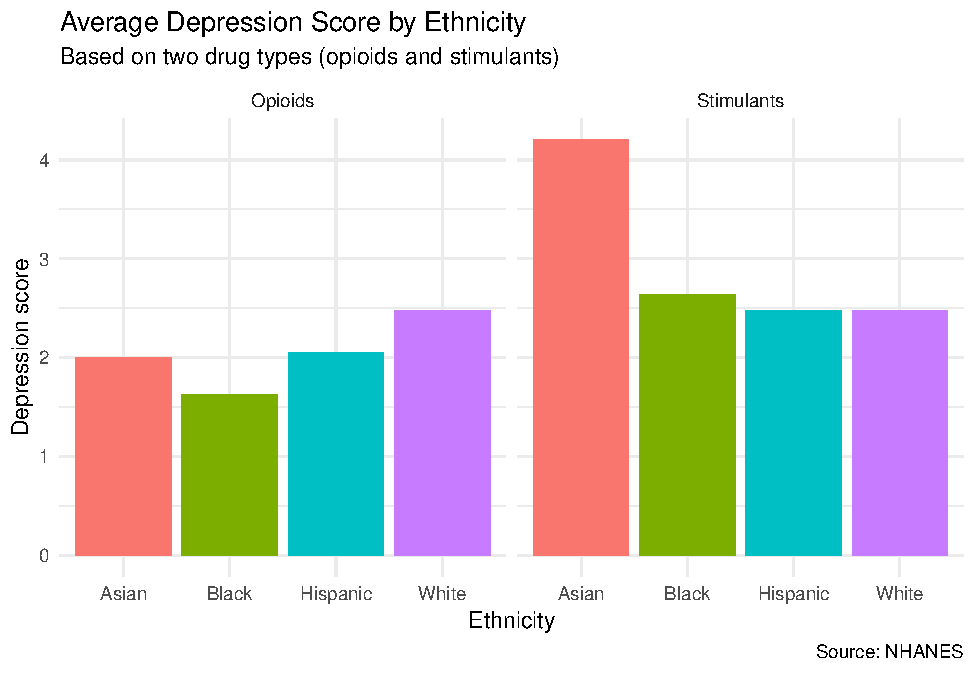
\includegraphics{Final_Paper_Group_3_files/figure-latex/ST_fig3-1.pdf}
\caption{}
\end{figure}

\begin{figure}
\centering
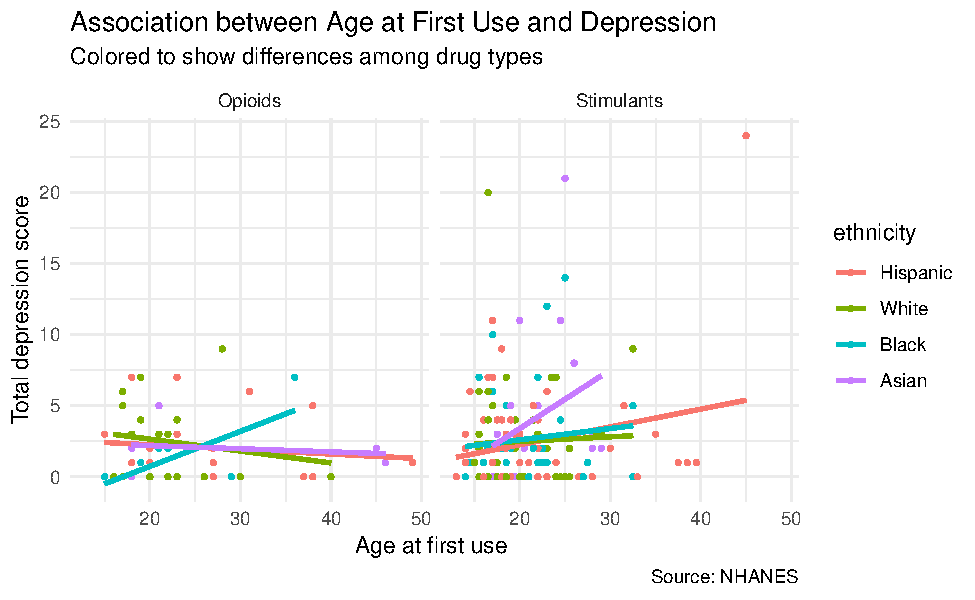
\includegraphics{Final_Paper_Group_3_files/figure-latex/ST_fig4-1.pdf}
\caption{}
\end{figure}

\subsection{Disparities in mental
health}\label{disparities-in-mental-health}

\begin{figure}
\centering
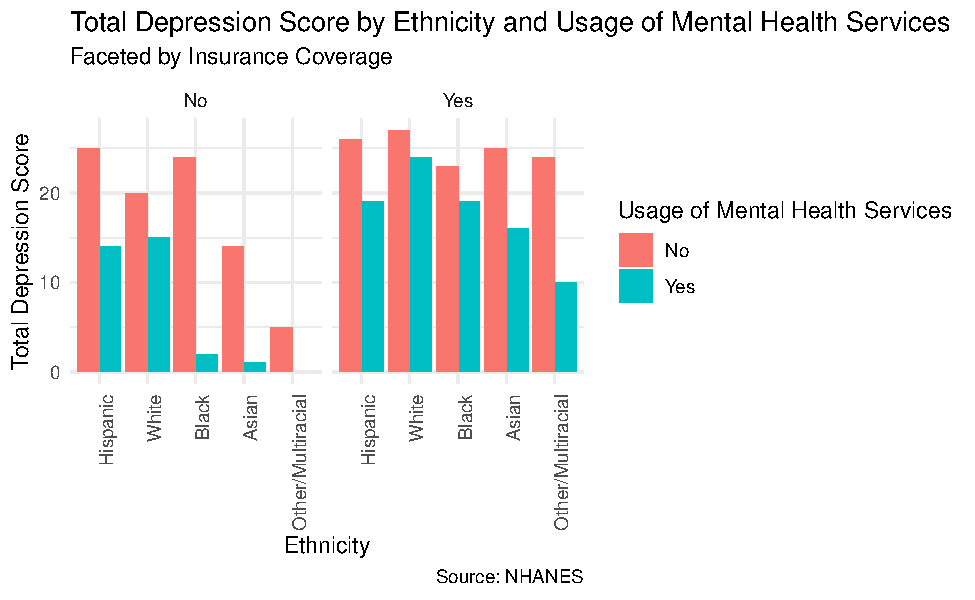
\includegraphics{Final_Paper_Group_3_files/figure-latex/AG_fig5-1.pdf}
\caption{}
\end{figure}

To investigate racial/ethnic disparities in mental health, we explored
insurance coverage and reported usage of mental health services (MHS) in
the last year by racial/ethnic group. As can be seen in Figure 5,
individuals who had insurance coverage had, on average, greater
depression scores than individuals who did not have insurance coverage.
Among individuals who did not have insurance coverage, the ones who
reported no usage of MHS in the last year had, on average, higher
depression scores than individuals who did report use of MHS in the last
year. Alternatively, the average depression score of individuals who had
insurance coverage did not differ substantially between individuals who
reported usage of MHS in the last year and individuals who reported no
usage of MHS in the last year. When looking at the differences between
racial/ethnic groups in regards to insurance coverage, we see that in
each racial/ethnic group there were more insured individuals than
uninsured individuals. However, when evaluating the percentages of
insured and uninsured individuals between each racial/ethnic group, the
differences were evident. For instance, the percentage of White
individuals who were insured, 92.48\%, was substantially higher than the
percentage of Hispanic individuals who were insured, 77.13\%. Among
uninsured individuals, Black and Asian individuals who used MHS in the
last year seemed to have much lower depression scores than their
uninsured counterparts who did not use MHS in the last year. On the
other hand, the discrepancy was much smaller between uninsured Hispanic
and White individuals who used MHS in the last year than those who did
not. In regards to insured individuals who reported use of MHS in the
last year and those who did not, the differences were not as significant
regardless of their racial/ethnic group, except for individuals who
identified as Other or Multiracial.

\section{Discussion}\label{discussion}

The results from this exploratory study provide a description of racial
and ethnic disparities based on recent date from a national U.S. sample
from 2015-2016. Strengths of this study include the nationally
representative sample, specifically exploring health disparities in
drugs have been overlooked until very recently (i.e., opioids and
stimulants), and identifying health disparities based on access to
adequate supports through insurance coverage. Results indicate that
having insurance coverage did not necessarily relate to lower depression
scores, in fact individuals who reported having insurance reported
higher depression scores, on average. This measure of insurance may not
have captured whether coverage was adequate, affordable, and if other
systemic factors such as a stigma, cultural values, or racism might have
affected depression outcomes. An additional limitation of this study, is
that the depression measure used in the NHANES study has not shown
evidence for cross-cultural validation, nor do we know if this measure
was administered in languages other than English. Finally, results
indicated that health disparities in opioid and stimulant drug use and
age of onset for first drug use exist in racial and ethnic minority
groups within the U. S. Hispanic individuals endorsed the greatest
levels of opioid and stimulant use and the most variability in onset of
drug use for both of these substances. Asian individuals reported the
lowest levels of opioid and stimulant use, which is in line with a
recent findings from the CDC (Disease Control et al., 2011). Future
studies should address the relationship between access to mental health
services and substance abuse treatment and age of onset, chronicity, and
frequency of drug use, as individuals may have alternate options when
struggling with mental health issues. Moreover, research on health
disparities is incomplete without the inclusion of systemic variables,
including socioeconomic conditions, and the perceived discrimination
within the systems that are intended to support prevention, treatment,
and rehabilitation of mental health conditions.

\newpage

\section{References}\label{references}

\begingroup
\setlength{\parindent}{-0.5in} \setlength{\leftskip}{0.5in}

\hypertarget{refs}{}
\hypertarget{ref-anthony2005drug}{}
Anthony, J. C., Chen, C. Y., \& Storr, C. L. (2005). Drug dependence
epidemiology. \emph{Clinical Neuroscience Research}, \emph{2}(5),
55--68.

\hypertarget{ref-R-papaja}{}
Aust, F., \& Barth, M. (2018). \emph{papaja: Create APA manuscripts with
R Markdown}. Retrieved from \url{https://github.com/crsh/papaja}

\hypertarget{ref-borowsky2000risk}{}
Borowsky, S. J., Rubenstein, L. V., Meredith, L. S., Camp, P.,
Jackson-Triche, M., \& Wells, K. B. (2000). Who is at risk of
nondetection of mental health problems in primary care? \emph{Journal of
General Internal Medicine}, \emph{15}(6), 381--388.

\hypertarget{ref-R-rio}{}
Chan, C.-h., Chan, G. C., Leeper, T. J., \& Becker, J. (2018).
\emph{Rio: A swiss-army knife for data file i/o}.

\hypertarget{ref-chen2005becomes}{}
Chen, C.-Y., O'Brien, M. S., \& Anthony, J. C. (2005). Who becomes
cannabis dependent soon after onset of use? Epidemiological evidence
from the united states: 2000--2001. \emph{Drug and Alcohol Dependence},
\emph{79}(1), 11--22.

\hypertarget{ref-centers2011cdc}{}
Disease Control, C. for, Prevention, \& others. (2011). CDC health
disparities and inequalities report: United states. \emph{Http://Www.
Cdc. Gov/Mmwr/Pdf/Other/Su6001. Pdf}.

\hypertarget{ref-fiscella2002disparities}{}
Fiscella, K., Franks, P., Doescher, M. P., \& Saver, B. G. (2002).
Disparities in health care by race, ethnicity, and language among the
insured: Findings from a national sample. \emph{Medical Care}, 52--59.

\hypertarget{ref-R-purrr}{}
Henry, L., \& Wickham, H. (2018). \emph{Purrr: Functional programming
tools}. Retrieved from \url{https://CRAN.R-project.org/package=purrr}

\hypertarget{ref-kroenke2001phq}{}
Kroenke, K., Spitzer, R. L., \& Williams, J. B. (2001). The phq-9:
Validity of a brief depression severity measure. \emph{Journal of
General Internal Medicine}, \emph{16}(9), 606--613.

\hypertarget{ref-levine2016black}{}
Levine, R. S., Foster, J. E., Fullilove, R. E., Fullilove, M. T.,
Briggs, N. C., Hull, P. C., \ldots{} Hennekens, C. H. (2016).
Black-white inequalities in mortality and life expectancy, 1933--1999:
Implications for healthy people 2010. \emph{Public Health Reports}.

\hypertarget{ref-miranda2004disparities}{}
Miranda, J., \& Cooper, L. A. (2004). Disparities in care for depression
among primary care patients. \emph{Journal of General Internal
Medicine}, \emph{19}(2), 120--126.

\hypertarget{ref-R-here}{}
Müller, K. (2017). \emph{Here: A simpler way to find your files}.
Retrieved from \url{https://CRAN.R-project.org/package=here}

\hypertarget{ref-R-bindrcpp}{}
Müller, K. (2018). \emph{Bindrcpp: An 'rcpp' interface to active
bindings}. Retrieved from
\url{https://CRAN.R-project.org/package=bindrcpp}

\hypertarget{ref-R-tibble}{}
Müller, K., \& Wickham, H. (2018). \emph{Tibble: Simple data frames}.
Retrieved from \url{https://CRAN.R-project.org/package=tibble}

\hypertarget{ref-R-base}{}
R Core Team. (2018). \emph{R: A language and environment for statistical
computing}. Vienna, Austria: R Foundation for Statistical Computing.
Retrieved from \url{https://www.R-project.org/}

\hypertarget{ref-who}{}
WHO. (2018). Depression. Retrieved from
\url{http://www.who.int/news-room/fact-sheets/detail/depression}

\hypertarget{ref-R-ggplot2}{}
Wickham, H. (2016). \emph{Ggplot2: Elegant graphics for data analysis}.
Springer-Verlag New York. Retrieved from \url{http://ggplot2.org}

\hypertarget{ref-R-tidyverse}{}
Wickham, H. (2017). \emph{Tidyverse: Easily install and load the
'tidyverse'}. Retrieved from
\url{https://CRAN.R-project.org/package=tidyverse}

\hypertarget{ref-R-forcats}{}
Wickham, H. (2018a). \emph{Forcats: Tools for working with categorical
variables (factors)}. Retrieved from
\url{https://CRAN.R-project.org/package=forcats}

\hypertarget{ref-R-stringr}{}
Wickham, H. (2018b). \emph{Stringr: Simple, consistent wrappers for
common string operations}. Retrieved from
\url{https://CRAN.R-project.org/package=stringr}

\hypertarget{ref-R-tidyr}{}
Wickham, H., \& Henry, L. (2018). \emph{Tidyr: Easily tidy data with
'spread()' and 'gather()' functions}. Retrieved from
\url{https://CRAN.R-project.org/package=tidyr}

\hypertarget{ref-R-dplyr}{}
Wickham, H., François, R., Henry, L., \& Müller, K. (2018). \emph{Dplyr:
A grammar of data manipulation}. Retrieved from
\url{https://CRAN.R-project.org/package=dplyr}

\hypertarget{ref-R-readr}{}
Wickham, H., Hester, J., \& Francois, R. (2018). \emph{Readr: Read
rectangular text data}. Retrieved from
\url{https://CRAN.R-project.org/package=readr}

\hypertarget{ref-williams2009discrimination}{}
Williams, D. R., \& Mohammed, S. A. (2009). Discrimination and racial
disparities in health: Evidence and needed research. \emph{Journal of
Behavioral Medicine}, \emph{32}(1), 20--47.

\hypertarget{ref-R-kableExtra}{}
Zhu, H. (n.d.). \emph{KableExtra: Construct complex table with 'kable'
and pipe syntax}.

\endgroup


\end{document}
